\chapter{THIẾT KẾ CHƯƠNG TRÌNH}

\section{Các chức năng chính}

\subsection{Đăng nhập hệ thống – F01 (\texorpdfstring{\code{Login\allowbreak{}Form.\allowbreak{}cs}}{LoginForm.cs})}

Màn hình đăng nhập không viền (borderless form) hỗ trợ kéo thả cửa sổ qua P/Invoke \code{user32.\allowbreak{}dll} (\code{Enable\allowbreak{}Drag}). Khi người dùng nhập tên đăng nhập và mật khẩu, sự kiện \code{Btn\allowbreak{}Login\_\allowbreak{}Click} kiểm tra dữ liệu rỗng, khóa tạm nút bấm (\code{Đang đăng nhập.\allowbreak{}.\allowbreak{}.\allowbreak{}}) và gọi bất đồng bộ \code{User\allowbreak{}Repository.\allowbreak{}Authenticate}. Hệ thống kiểm tra tài khoản tồn tại, đối chiếu mật khẩu băm qua \code{Password\allowbreak{}Hasher.\allowbreak{}Verify}, kiểm tra cờ hoạt động \code{Is\allowbreak{}Active = 1}, sau đó nạp danh sách mã quyền từ bảng \code{Role\allowbreak{}Permissions} vào \code{Session.\allowbreak{}Start} trước khi mở \code{Main\allowbreak{}Form}.


\subsection{Quản lý tài khoản và đặt lại mật khẩu – F04 (\texorpdfstring{\code{User\allowbreak{}Page.\allowbreak{}cs}}{UserPage.cs})}

Dành cho người dùng có quyền \code{USER\_\allowbreak{}MANAGE}. Cho phép tìm kiếm tài khoản theo tên đăng nhập, họ tên hoặc email; thêm mới tài khoản (\code{User\allowbreak{}Edit\allowbreak{}Dialog}), cập nhật thông tin cá nhân và nhóm quyền, khóa hoặc mở khóa tài khoản (\code{Set\allowbreak{}User\allowbreak{}Active}) và đặt lại mật khẩu (\code{Password\allowbreak{}Reset\allowbreak{}Dialog}). Presenter \code{Admin\allowbreak{}Service} kiểm tra độ dài tên đăng nhập (3–50 ký tự), mật khẩu tối thiểu 8 ký tự, và chặn thao tác tự khóa chính tài khoản đang đăng nhập (\code{id == current\allowbreak{}User\allowbreak{}Id}).


\subsection{Quản lý nhóm quyền và phân quyền – F05 (\texorpdfstring{\code{Role\allowbreak{}Page.\allowbreak{}cs}}{RolePage.cs})}

Dành cho người quản lý có quyền \code{ROLE\_\allowbreak{}MANAGE}. Giao diện chia hai cột bằng \code{Split\allowbreak{}Container}: cột trái hiển thị danh sách nhóm quyền (\code{Roles}) kèm số lượng tài khoản thuộc nhóm, cho phép thêm mới hoặc đổi tên/mô tả nhóm quyền (\code{Role\allowbreak{}Edit\allowbreak{}Dialog}); cột phải hiển thị danh sách 17 quyền chức năng dưới dạng \code{Checked\allowbreak{}List\allowbreak{}Box}. Khi nhấn \code{Lưu quyền}, phương thức \code{Admin\allowbreak{}Repository.\allowbreak{}Save\allowbreak{}Role\allowbreak{}Permissions} thực thi trong một transaction để xóa tập quyền cũ và chèn tập quyền mới cho nhóm được chọn.


\subsection{Màn hình chính và Dashboard – F02 (\texorpdfstring{\code{Main\allowbreak{}Form.\allowbreak{}cs}}{MainForm.cs}, \texorpdfstring{\code{Dashboard\allowbreak{}Page.\allowbreak{}cs}}{DashboardPage.cs})}

Khung chính \code{Main\allowbreak{}Form} tự động dựng thanh điều hướng bên trái (\code{Build\allowbreak{}Nav}) dựa trên danh mục \code{Nav\allowbreak{}Catalog.\allowbreak{}Items}, chỉ hiển thị những mục mà phiên làm việc hiện tại có quyền truy cập, được gom theo 4 phân nhóm: Tổng quan, Danh mục, Mượn trả, Báo cáo và Hệ thống. Trang mặc định \code{Dashboard\allowbreak{}Page} (F02) hiển thị 4 thẻ chỉ số trực quan (\code{Stat\allowbreak{}Card}) gồm: Tổng số đầu thiết bị đang hoạt động, Tổng số đơn vị khả dụng, Số phiếu đang mượn và Số phiếu quá hạn; phía dưới là bảng 8 phiếu mượn gần nhất kèm nhãn màu trạng thái.


\subsection{Quản lý loại thiết bị – F06 (\texorpdfstring{\code{Category\allowbreak{}Page.\allowbreak{}cs}}{CategoryPage.cs})}

Hiển thị danh mục phân loại thiết bị (như \code{LAPTOP}, \code{PROJ}, \code{CAM}, \code{AUDIO}, \code{NET}, \code{OTHER}) kèm số lượng thiết bị đang hoạt động thuộc mỗi loại. Nhân viên kho chỉ có quyền \code{CATEGORY\_\allowbreak{}VIEW} nên các nút Thêm, Sửa, Xóa tự động ẩn trên giao diện. Người quản lý có quyền \code{CATEGORY\_\allowbreak{}MANAGE} được phép thêm/sửa loại thiết bị (mã loại tự động chuẩn hóa chữ in hoa, chỉ nhận chữ không dấu, số, gạch ngang/dưới) và chỉ xóa được loại thiết bị khi chưa có thiết bị nào tham chiếu tới.


\subsection{Quản lý thiết bị và tồn kho – F07 (\texorpdfstring{\code{Device\allowbreak{}Page.\allowbreak{}cs}}{DevicePage.cs})}

Quản lý thông tin chi tiết từng thiết bị: mã thiết bị, tên thiết bị, loại thiết bị, đơn vị tính, tổng số lượng (\code{Total\allowbreak{}Quantity}), khả dụng (\code{Available\allowbreak{}Quantity}), đang mượn (\code{On\allowbreak{}Loan\allowbreak{}Quantity}), hư hỏng (\code{Damaged\allowbreak{}Quantity}) và mất (\code{Lost\allowbreak{}Quantity}). Hỗ trợ tìm kiếm có trễ (debounce timer 350ms) và lọc theo loại thiết bị. Khi thêm mới, hệ thống gợi ý mã tự động (\code{TB0009.\allowbreak{}.\allowbreak{}.\allowbreak{}}). Khi cập nhật tổng số lượng, hệ thống tự động cộng/trừ phần chênh lệch vào số lượng khả dụng và ngăn giảm tổng số lượng xuống thấp hơn tổng số đang mượn cộng hư hỏng/mất. Ngoài ra, \code{Device\allowbreak{}Service.\allowbreak{}Recover\allowbreak{}Damaged} hỗ trợ chuyển số lượng thiết bị hư hỏng đã sửa chữa xong quay về nhóm khả dụng.


\subsection{Quản lý người mượn và lịch sử – F08 (\texorpdfstring{\code{Borrower\allowbreak{}Page.\allowbreak{}cs}}{BorrowerPage.cs})}

Lưu trữ hồ sơ người mượn (\code{Borrower\allowbreak{}Code}, họ tên, điện thoại, email, phòng ban/đơn vị, địa chỉ, ghi chú và trạng thái hoạt động). \code{Borrower\allowbreak{}Service} kiểm tra định dạng số điện thoại và email bằng biểu thức chính quy biên dịch sẵn (\code{Generated\allowbreak{}Regex}). Người dùng có thể lọc xem cả người mượn đã ngừng hoạt động, mở hộp thoại \code{Borrower\allowbreak{}History\allowbreak{}Dialog} để tra cứu toàn bộ lịch sử phiếu mượn của người đó, hoặc xóa hồ sơ nếu người mượn chưa từng phát sinh phiếu mượn nào.


\subsection{Lập phiếu mượn nhiều thiết bị – F09 (\texorpdfstring{\code{Loan\allowbreak{}Create\allowbreak{}Page.\allowbreak{}cs}}{LoanCreatePage.cs})}

Màn hình chia đôi gồm danh sách thiết bị còn khả dụng bên trái và giỏ thiết bị chọn mượn (\code{Cart\allowbreak{}Row}) bên phải. Nhân viên chọn người mượn, ngày mượn, hạn dự kiến trả và thêm một hoặc nhiều thiết bị vào phiếu; nếu chọn trùng thiết bị đã có trong giỏ thì hệ thống tự động cộng dồn số lượng và đối chiếu không vượt quá \code{Available\allowbreak{}Quantity}. Khi nhấn \code{Lưu phiếu mượn}, \code{Loan\allowbreak{}Service.\allowbreak{}Create} thực thi trong một SQL Transaction: kiểm tra người mượn đang hoạt động, gọi \code{sp\_\allowbreak{}Get\allowbreak{}Next\allowbreak{}Code} sinh mã phiếu (\code{PM-\allowbreak{}yyyy\allowbreak{}MMdd-\allowbreak{}xxxx}), tạo đầu phiếu \code{Loan\allowbreak{}Slips}, trừ tồn kho có điều kiện và lưu từng dòng \code{Loan\allowbreak{}Slip\allowbreak{}Details}.


\subsection{Tra cứu và xem chi tiết phiếu mượn – F10, F11 (\texorpdfstring{\code{Loan\allowbreak{}Search\allowbreak{}Page.\allowbreak{}cs}}{LoanSearchPage.cs})}

Cho phép tìm kiếm phiếu mượn theo từ khóa (mã phiếu, tên/mã người mượn, số điện thoại), lọc theo khoảng ngày mượn, khoảng hạn trả và 4 trạng thái hiển thị (\code{Đang mượn}, \code{Trả một phần}, \code{Đã trả}, \code{Quá hạn}). Khi nhấp đúp hoặc nhấn \code{Xem chi tiết}, hộp thoại \code{Loan\allowbreak{}Slip\allowbreak{}Detail\allowbreak{}Dialog} (F11) hiển thị đầy đủ thông tin đầu phiếu và 2 tab: danh sách thiết bị trong phiếu (số lượng mượn, đã trả, còn lại) và lịch sử tất cả các biên bản trả của phiếu đó.


\subsection{Ghi nhận trả thiết bị theo tình trạng – F12 (\texorpdfstring{\code{Return\allowbreak{}Create\allowbreak{}Page.\allowbreak{}cs}}{ReturnCreatePage.cs})}

Liệt kê danh sách các phiếu mượn còn số lượng thiết bị chưa trả (\code{Remaining\allowbreak{}Qty \textgreater{} 0}). Khi chọn một phiếu và mở \code{Return\allowbreak{}Create\allowbreak{}Dialog}, nhân viên nhập ngày trả, tên người giao và điền số lượng trả cho từng thiết bị kèm tình trạng bàn giao (\code{Tốt}, \code{Hư hỏng}, \code{Mất}, \code{Thiếu phụ kiện}) và ghi chú. Nếu chọn tình trạng \code{Hư hỏng} hoặc \code{Thiếu phụ kiện}, hệ thống bắt buộc phải nhập ghi chú mô tả chi tiết trước khi lưu.


\subsection{Tra cứu, xem và hủy biên bản trả – F13 (\texorpdfstring{\code{Return\allowbreak{}Record\allowbreak{}Page.\allowbreak{}cs}}{ReturnRecordPage.cs})}

Quản lý danh sách biên bản bàn giao trả thiết bị (\code{BB-\allowbreak{}yyyy\allowbreak{}MMdd-\allowbreak{}xxxx}), lọc theo từ khóa, khoảng ngày trả và trạng thái (\code{Hiệu lực} / \code{Đã hủy}). Hộp thoại \code{Return\allowbreak{}Record\allowbreak{}Detail\allowbreak{}Dialog} hiển thị chi tiết từng dòng thiết bị đã trả và cho phép xem trước/in biên bản. Đối với tài khoản có quyền \code{RECORD\_\allowbreak{}CANCEL}, nút \code{Hủy biên bản} cho phép nhập lý do hủy để hoàn tác số lượng đã trả trên phiếu mượn và trừ ngược lại đúng nhóm tồn kho đã cộng trước đó mà không xóa cứng bản ghi.


\subsection{Danh sách phiếu quá hạn – F14 (\texorpdfstring{\code{Overdue\allowbreak{}Page.\allowbreak{}cs}}{OverduePage.cs})}

Gọi thủ tục lưu trữ \code{dbo.\allowbreak{}sp\_\allowbreak{}Get\allowbreak{}Overdue\allowbreak{}Slips} để truy xuất các phiếu mượn đã quá ngày hạn trả (\code{Due\allowbreak{}Date \textless{} As\allowbreak{}Of\allowbreak{}Date}) nhưng vẫn còn thiết bị chưa trả đủ. Màn hình hỗ trợ tìm kiếm theo mã phiếu, tên hoặc số điện thoại người mượn, lọc theo số ngày trễ tối thiểu, đồng thời hiển thị cột tổng hợp danh sách tên và số lượng từng thiết bị đang nợ (\code{Unreturned\allowbreak{}Devices}).


\subsection{Báo cáo, thống kê top thiết bị và in ấn – F15, F18 (\texorpdfstring{\code{Report\allowbreak{}Page.\allowbreak{}cs}}{ReportPage.cs})}

Trang \code{Report\allowbreak{}Page} (F15) thống kê theo khoảng ngày: tổng số phiếu mượn, tổng số lượng mượn, đã trả, còn phải trả, số phiếu quá hạn và bức tranh tồn kho hiện tại (số đầu thiết bị hoạt động, khả dụng, hư hỏng, mất). Hệ thống phân tách rõ quyền \code{REPORT\_\allowbreak{}PRINT} (chỉ được in phiếu/biên bản) và quyền \code{REPORT\_\allowbreak{}VIEW} (được xem số liệu báo cáo tổng hợp). Trang \code{Popular\allowbreak{}Device\allowbreak{}Page} (F18) xếp hạng Top N thiết bị được mượn nhiều nhất theo tổng số lượng mượn giảm dần.


\subsection{Cấu hình mã tự động và giao diện sáng/tối – F16 (\texorpdfstring{\code{Code\allowbreak{}Config\allowbreak{}Page.\allowbreak{}cs}}{CodeConfigPage.cs})}

Trang \code{Code\allowbreak{}Config\allowbreak{}Page} (F16) cho phép người quản lý cấu hình quy tắc sinh mã cho 4 thực thể (\code{Loan\allowbreak{}Slip}, \code{Return\allowbreak{}Record}, \code{Device}, \code{Borrower}) gồm: tiền tố (\code{Prefix}), độ dài phần số (\code{Number\allowbreak{}Length} từ 1–9), tùy chọn chèn ngày (\code{Use\allowbreak{}Date}) và đặt lại bộ đếm hằng ngày (\code{Reset\allowbreak{}Daily}), kèm nút \code{Xem mã tiếp theo} (\code{Peek}). Ngoài ra, nút chuyển đổi giao diện Sáng/Tối trên thanh tiêu đề \code{Main\allowbreak{}Form} gọi \code{Theme.\allowbreak{}Toggle()} giúp toàn bộ Form và control tự động vẽ lại bảng màu tức thời.


\section{Thiết kế cơ sở dữ liệu chương trình}

\subsection{Sơ đồ quan hệ ERD}

Cơ sở dữ liệu \code{Quan\allowbreak{}Ly\allowbreak{}Muon\allowbreak{}Tra} được thiết kế gồm 12 bảng dữ liệu chuẩn hóa, chia thành 3 phân khu: Phân quyền \& Người dùng (\code{Roles}, \code{Permissions}, \code{Role\allowbreak{}Permissions}, \code{Users}), Danh mục \& Cấu hình (\code{Device\allowbreak{}Categories}, \code{Devices}, \code{Borrowers}, \code{Code\allowbreak{}Configs}) và Giao dịch Mượn – Trả (\code{Loan\allowbreak{}Slips}, \code{Loan\allowbreak{}Slip\allowbreak{}Details}, \code{Return\allowbreak{}Records}, \code{Return\allowbreak{}Record\allowbreak{}Details}). Hình 3.1 dưới đây biểu diễn sơ đồ quan hệ thực thể được trích xuất trực tiếp từ các tệp \code{Database/\allowbreak{}02\_\allowbreak{}Create\allowbreak{}Tables.\allowbreak{}sql} và \code{03\_\allowbreak{}Constraints.\allowbreak{}sql}.


\begin{figure}[H]\centering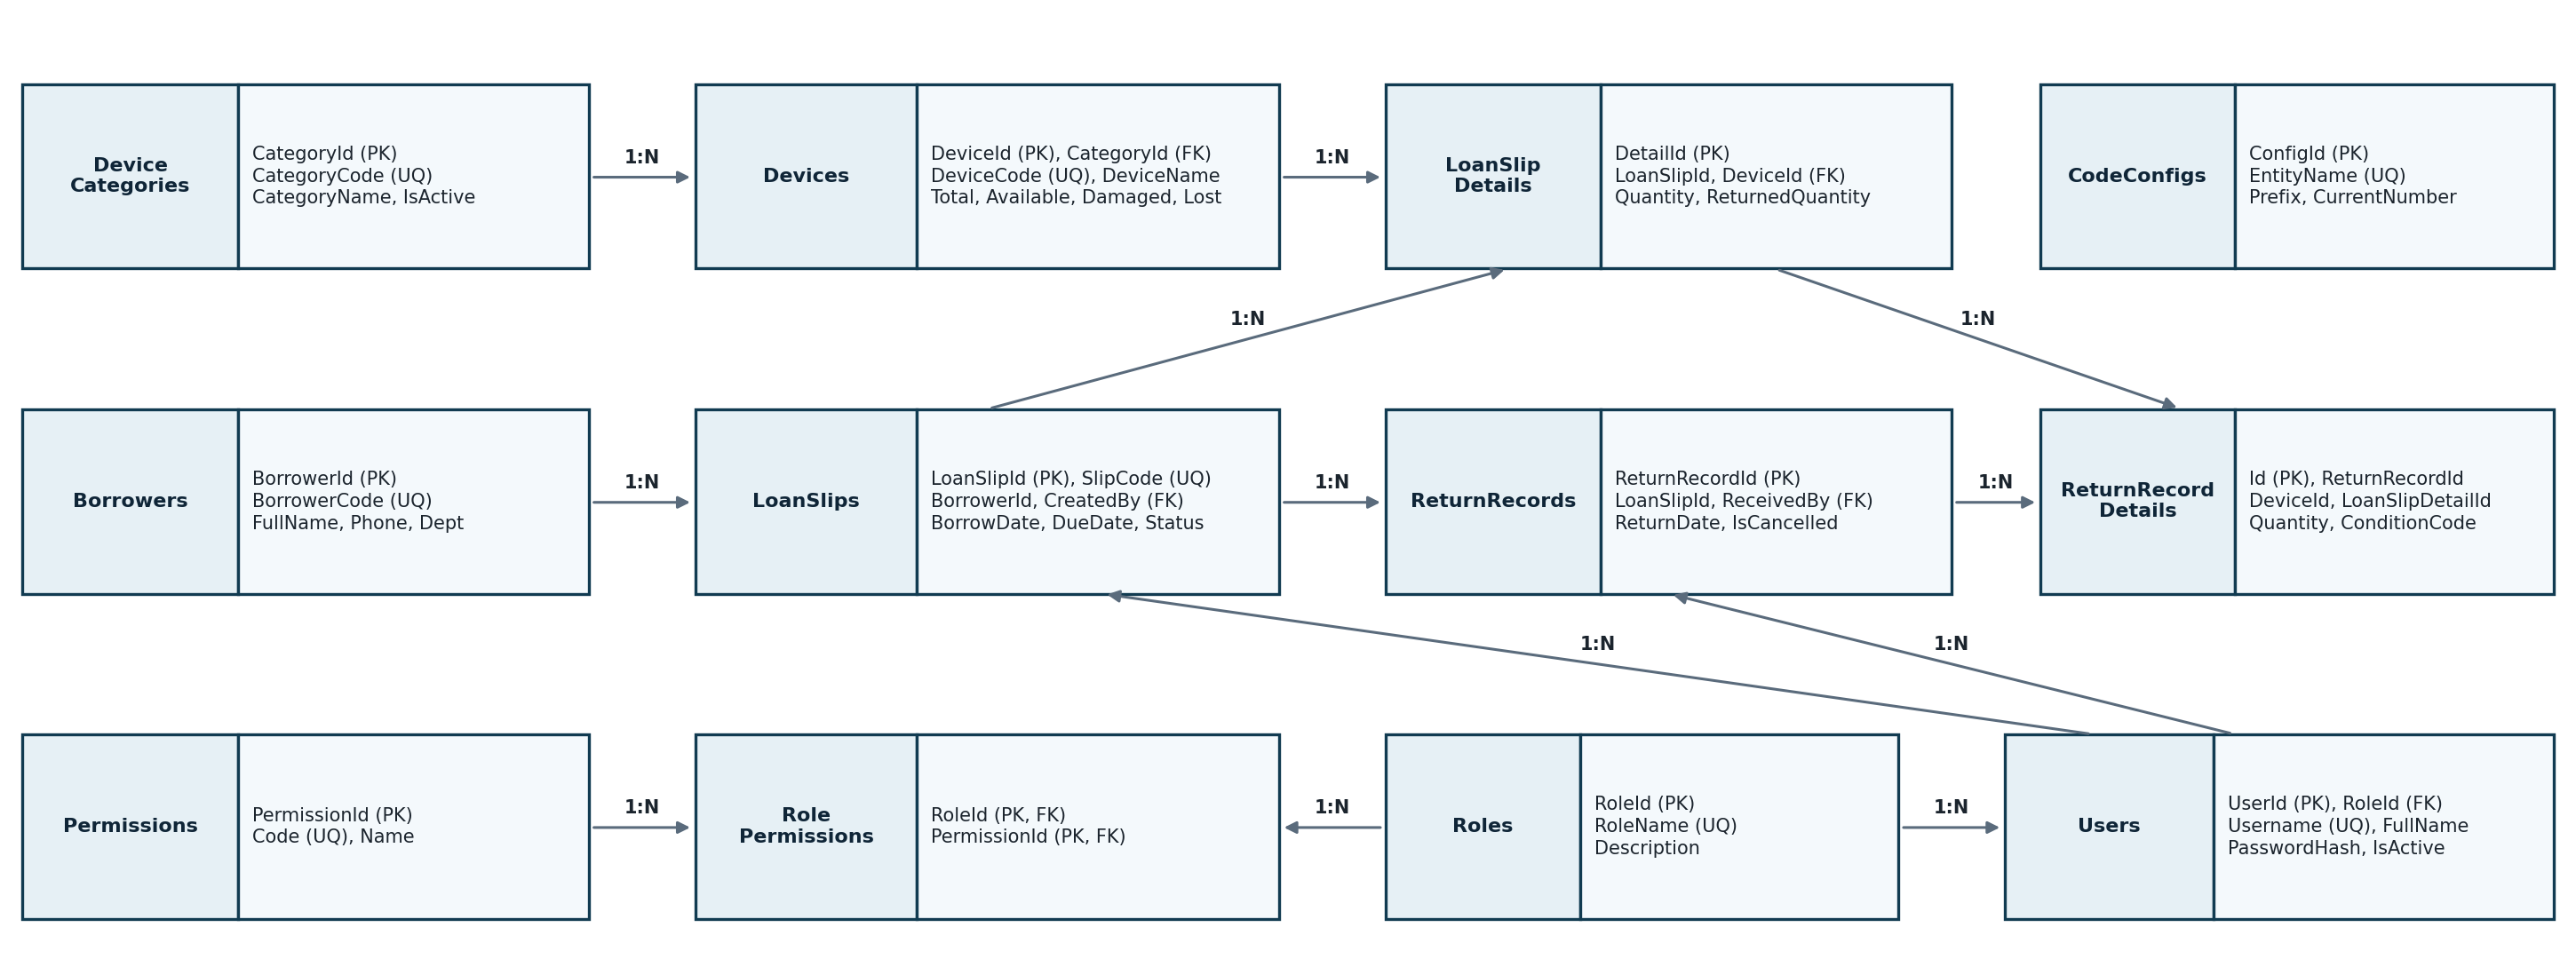
\includegraphics[width=0.8\linewidth]{images/image20.png}\caption{Sơ đồ quan hệ thực thể (ERD) hệ thống Quản lý mượn trả thiết bị}\end{figure}

\subsection{Mô tả chi tiết các bảng dữ liệu}

{\small\setlength{\tabcolsep}{3pt}\renewcommand{\arraystretch}{1.25}
\begin{longtable}{|>{\raggedright\arraybackslash}p{0.114\linewidth}|>{\raggedright\arraybackslash}p{0.133\linewidth}|>{\raggedright\arraybackslash}p{0.361\linewidth}|>{\raggedright\arraybackslash}p{0.361\linewidth}|}
\caption{Tóm tắt 12 bảng dữ liệu chính}\\
\hline
\rowcolor{gray!25}\textbf{\textbf{Bảng}} & \textbf{\textbf{Khóa chính}} & \textbf{\textbf{Trường tiêu biểu}} & \textbf{\textbf{Ý nghĩa}} \\ \hline
\endfirsthead
\hline
\rowcolor{gray!25}\textbf{\textbf{Bảng}} & \textbf{\textbf{Khóa chính}} & \textbf{\textbf{Trường tiêu biểu}} & \textbf{\textbf{Ý nghĩa}} \\ \hline
\endhead
\hline\endfoot
Roles & RoleId & RoleName (UQ), Description & Lưu danh sách vai trò/nhóm quyền trong hệ thống. \\ \hline
Permissions & PermissionId & Code (UQ), Name & Danh mục 17 mã quyền chức năng chuẩn của phần mềm. \\ \hline
RolePermissions & (RoleId, PermissionId) & RoleId (FK), PermissionId (FK) & Bảng trung gian ánh xạ quan hệ nhiều–nhiều giữa vai trò và quyền. \\ \hline
Users & UserId & Username (UQ), PasswordHash, FullName, RoleId (FK), IsActive & Lưu tài khoản nhân viên kho và người quản lý; mật khẩu băm PBKDF2. \\ \hline
DeviceCategories & CategoryId & CategoryCode (UQ), CategoryName, Description, IsActive & Danh mục phân loại trang thiết bị (Laptop, Máy chiếu, Âm thanh...). \\ \hline
Devices & DeviceId & DeviceCode (UQ), DeviceName, CategoryId (FK), TotalQuantity, AvailableQuantity, DamagedQuantity, LostQuantity & Quản lý thiết bị và cân bằng 4 nhóm số lượng tồn kho. \\ \hline
Borrowers & BorrowerId & BorrowerCode (UQ), FullName, Phone, Email, Department, Address, IsActive & Hồ sơ thông tin liên hệ và đơn vị công tác của người mượn. \\ \hline
LoanSlips & LoanSlipId & SlipCode (UQ), BorrowerId (FK), CreatedBy (FK), BorrowDate, DueDate, Status & Đầu phiếu mượn thiết bị (Status: 0 = còn nợ, 1 = đã trả đủ). \\ \hline
LoanSlipDetails & DetailId & LoanSlipId (FK), DeviceId (FK), Quantity, ReturnedQuantity & Chi tiết từng thiết bị và tiến độ số lượng đã trả trong phiếu mượn. \\ \hline
ReturnRecords & ReturnRecordId & RecordCode (UQ), LoanSlipId (FK), ReturnDate, ReceivedBy (FK), GiverName, IsCancelled, CancelledBy, CancelReason & Đầu biên bản trả/bàn giao thiết bị và thông tin truy vết hủy biên bản. \\ \hline
ReturnRecordDetails & Id & ReturnRecordId (FK), DeviceId (FK), LoanSlipDetailId (FK), Quantity, ConditionCode, Condition & Chi tiết số lượng và tình trạng thiết bị trong từng lần trả (0..3). \\ \hline
CodeConfigs & ConfigId & EntityName (UQ), Prefix, UseDate, NumberLength, CurrentNumber, ResetDaily, LastResetDate & Quy tắc và bộ đếm sinh mã tự động cho từng đối tượng. \\ \hline
\end{longtable}
}

Hệ thống thiết lập các ràng buộc toàn vẹn chặt chẽ trong \code{03\_\allowbreak{}Constraints.\allowbreak{}sql}: ràng buộc \code{CK\_\allowbreak{}Devices\_\allowbreak{}Inventory} bảo đảm \code{Available\allowbreak{}Quantity \textgreater{}= 0}, \code{Damaged\allowbreak{}Quantity \textgreater{}= 0}, \code{Lost\allowbreak{}Quantity \textgreater{}= 0} và \code{Available\allowbreak{}Quantity + Damaged\allowbreak{}Quantity + Lost\allowbreak{}Quantity \textless{}= Total\allowbreak{}Quantity}; ràng buộc \code{CK\_\allowbreak{}Loan\allowbreak{}Slip\allowbreak{}Details\_\allowbreak{}Returned} kiểm soát \code{0 \textless{}= Returned\allowbreak{}Quantity \textless{}= Quantity}; ràng buộc \code{CK\_\allowbreak{}Loan\allowbreak{}Slips\_\allowbreak{}Dates} kiểm tra \code{Due\allowbreak{}Date \textgreater{}= Borrow\allowbreak{}Date}; ràng buộc \code{CK\_\allowbreak{}RRD\_\allowbreak{}Condition\allowbreak{}Code} giới hạn mã tình trạng trong tập \code{(0, 1, 2, 3)}; và ràng buộc \code{CK\_\allowbreak{}Code\allowbreak{}Configs\_\allowbreak{}Rules} bắt buộc \code{Reset\allowbreak{}Daily = 0 OR Use\allowbreak{}Date = 1} để ngăn việc đặt lại bộ đếm mỗi ngày khi mã không đính kèm ngày tháng. Bên cạnh đó, chỉ mục duy nhất \code{UQ\_\allowbreak{}Loan\allowbreak{}Slip\allowbreak{}Details\_\allowbreak{}Slip\_\allowbreak{}Device} ngăn một thiết bị xuất hiện lặp lại trên hai dòng của cùng một phiếu mượn, và 14 chỉ mục non-clustered trong \code{04\_\allowbreak{}Indexes.\allowbreak{}sql} giúp tối ưu tốc độ tìm kiếm, lọc và nối bảng.


\subsection{View, Stored procedure và transaction}

{\small\setlength{\tabcolsep}{3pt}\renewcommand{\arraystretch}{1.25}
\begin{longtable}{|>{\raggedright\arraybackslash}p{0.233\linewidth}|>{\raggedright\arraybackslash}p{0.155\linewidth}|>{\raggedright\arraybackslash}p{0.582\linewidth}|}
\caption{Các View và Stored Procedure trong cơ sở dữ liệu}\\
\hline
\rowcolor{gray!25}\textbf{\textbf{Đối tượng SQL}} & \textbf{\textbf{Loại}} & \textbf{\textbf{Mục đích và cơ chế xử lý}} \\ \hline
\endfirsthead
\hline
\rowcolor{gray!25}\textbf{\textbf{Đối tượng SQL}} & \textbf{\textbf{Loại}} & \textbf{\textbf{Mục đích và cơ chế xử lý}} \\ \hline
\endhead
\hline\endfoot
vw\_LoanSlipSummary & View & Tổng hợp đầu phiếu mượn, thông tin người mượn, người lập, tổng số lượng mượn (TotalQty), đã trả (ReturnedQty), còn lại (RemainingQty), số ngày trễ (DaysOverdue) và tự động suy diễn trạng thái hiển thị DisplayStatus (0: Đang mượn, 1: Trả một phần, 2: Đã trả, 3: Quá hạn). \\ \hline
sp\_GetNextCode & Stored Procedure & Sinh mã tự động theo bảng CodeConfigs. Sử dụng gợi ý khóa dòng WITH (UPDLOCK, HOLDLOCK) trong transaction để nhiều người dùng thao tác cùng lúc không bao giờ sinh trùng mã; hỗ trợ chế độ @Peek = 1 để xem trước mã mà không tăng bộ đếm. \\ \hline
sp\_GetOverdueSlips & Stored Procedure & Truy vấn danh sách phiếu quá hạn thực tế theo ngày (@AsOfDate), hỗ trợ lọc từ khóa (@Keyword) và số ngày quá hạn tối thiểu (@MinDaysOverdue), đồng thời dùng CROSS APPLY + STRING\_AGG để nối danh sách tên thiết bị và số lượng chưa trả. \\ \hline
sp\_RecalculateInventory & Stored Procedure & Đồng bộ lại trạng thái phiếu mượn (LoanSlips.Status) và tính lại tồn kho khả dụng chuẩn xác theo công thức Available = Total - (Đang mượn) - Damaged - Lost; dùng sau khi nạp dữ liệu mẫu hoặc khi cần đối soát dữ liệu. \\ \hline
\end{longtable}
}

\section{Kiến trúc và luồng xử lý}

Ứng dụng được tổ chức thành 2 project trong cùng một solution: \code{Quan\allowbreak{}Ly\allowbreak{}Muon\allowbreak{}Tra.\allowbreak{}UI} (thư viện control và chủ đề giao diện) và \code{Quan\allowbreak{}Ly\allowbreak{}Muon\allowbreak{}Tra.\allowbreak{}App} (chứa các phân lớp \code{Forms}/\code{Pages}, \code{Services}, \code{Data}, \code{Models}, \code{Security}). Hình 3.2 minh họa kiến trúc MVP và mối liên hệ giữa các thành phần và Hình 3.3 thể hiện luồng xử lý nghiệp vụ mượn – trả thiết bị khép kín.


\begin{figure}[H]\centering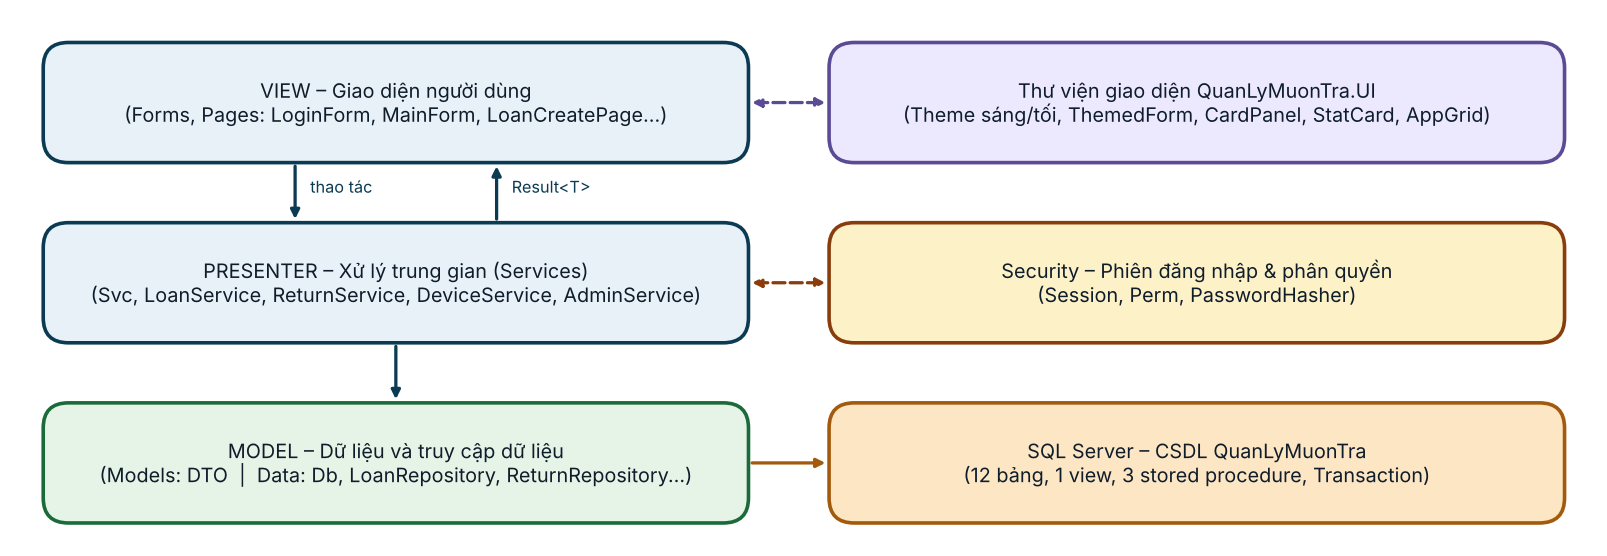
\includegraphics[width=0.8\linewidth]{images/image21.png}\caption{Mô hình kiến trúc MVP (Model – View – Presenter), SQL Server và thư viện UI}\end{figure}

\begin{figure}[H]\centering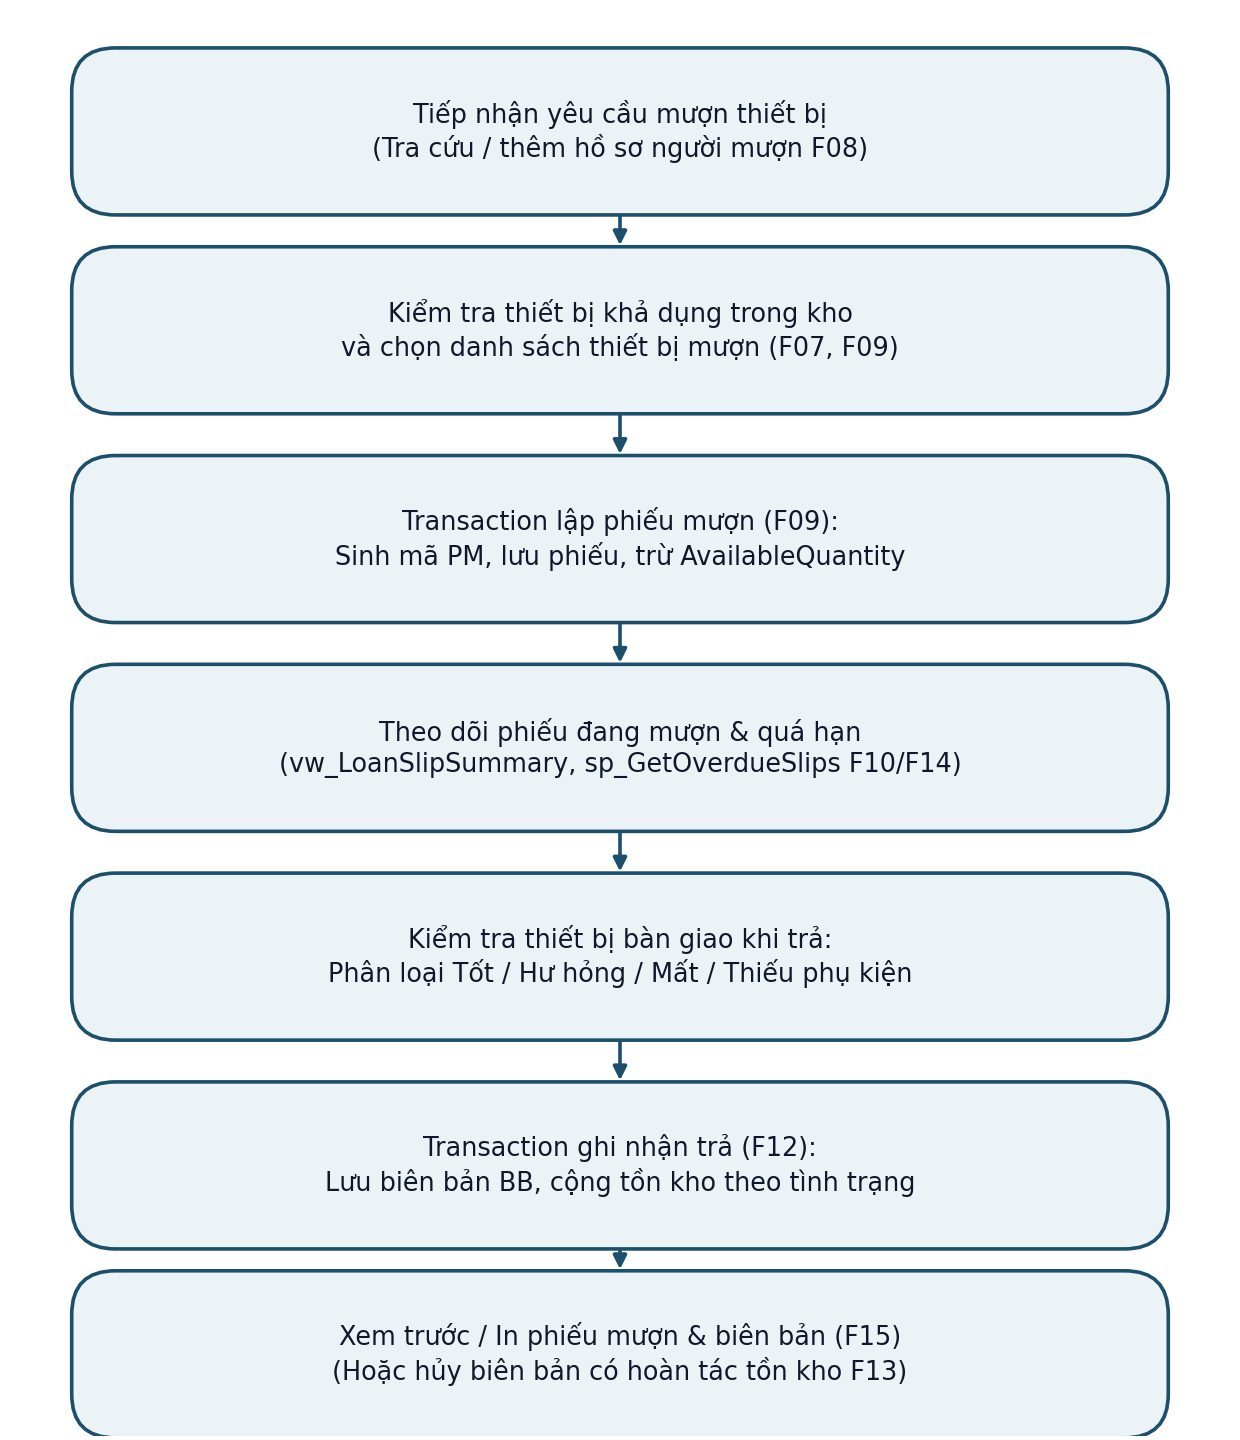
\includegraphics[width=0.8\linewidth]{images/image22.png}\caption{Quy trình nghiệp vụ từ lập phiếu mượn đến ghi nhận trả và in biên bản}\end{figure}

\section{Quy tắc nghiệp vụ và kiểm soát tồn kho}

Khác với bài toán bán hàng thông thường, bài toán quản lý mượn trả thiết bị đòi hỏi bảo toàn tổng số lượng tài sản đầu tư trong suốt vòng đời cho mượn, trả lại, hư hỏng, sửa chữa hoặc thất lạc. Các công thức bất biến được duy trì xuyên suốt giữa tầng C\# (\code{Loan\allowbreak{}Repository.\allowbreak{}cs}, \code{Return\allowbreak{}Repository.\allowbreak{}cs}) và tầng SQL Server (\code{03\_\allowbreak{}Constraints.\allowbreak{}sql}, \code{05\_\allowbreak{}Stored\allowbreak{}Procedures.\allowbreak{}sql}):


\begin{Verbatim}
ĐangMượn (OnLoanQuantity) = Σ (Quantity - ReturnedQuantity) trên LoanSlipDetails
TổngSốLượng (TotalQuantity) = AvailableQuantity + OnLoanQuantity + DamagedQuantity + LostQuantity
CònPhảiTrả (RemainingQty) = TotalQty - ReturnedQty (trên từng dòng và toàn phiếu)
SốNgàyQuáHạn (DaysOverdue) = max(0, (HômNay - DueDate).Days) khi RemainingQty > 0 và DueDate < HômNay
\end{Verbatim}

Khi ghi nhận trả thiết bị tại \code{Return\allowbreak{}Repository.\allowbreak{}Create}, phương thức phân loại \code{Bucket(condition\allowbreak{}Code, qty)} quy đổi số lượng trả vào 3 rổ tồn kho \code{(Good, Damaged, Lost)} theo đúng mã tình trạng: nếu trả ở tình trạng \textbf{Tốt (\code{0})}, số lượng được cộng trả lại vào \code{Available\allowbreak{}Quantity} để sẵn sàng cho lượt mượn tiếp theo; nếu trả ở tình trạng \textbf{Hư hỏng (\code{1})} hoặc \textbf{Thiếu phụ kiện (\code{3})}, số lượng được cộng vào \code{Damaged\allowbreak{}Quantity} (chờ sửa chữa/bổ sung phụ kiện qua \code{Recover\allowbreak{}Damaged}); nếu trả ở tình trạng \textbf{Mất (\code{2})}, số lượng được cộng vào \code{Lost\allowbreak{}Quantity}. Trạng thái hiển thị \code{Display\allowbreak{}Status} của phiếu mượn không lưu cứng mà được tính động trên \code{vw\_\allowbreak{}Loan\allowbreak{}Slip\allowbreak{}Summary}: ưu tiên kiểm tra nếu \code{Remaining\allowbreak{}Qty = 0} là \code{Đã trả (2)}, ngược lại nếu \code{Due\allowbreak{}Date \textless{} Hôm\allowbreak{}Nay} là \code{Quá hạn (3)}, nếu \code{Returned\allowbreak{}Qty \textgreater{} 0} là \code{Trả một phần (1)}, và mặc định là \code{Đang mượn (0)}.


{\small\setlength{\tabcolsep}{3pt}\renewcommand{\arraystretch}{1.25}
\begin{longtable}{|>{\raggedright\arraybackslash}p{0.485\linewidth}|>{\raggedright\arraybackslash}p{0.485\linewidth}|}
\caption{Các tình huống kiểm soát nghiệp vụ}\\
\hline
\rowcolor{gray!25}\textbf{\textbf{Tình huống nghiệp vụ}} & \textbf{\textbf{Cơ chế kiểm soát và kết quả kỳ vọng}} \\ \hline
\endfirsthead
\hline
\rowcolor{gray!25}\textbf{\textbf{Tình huống nghiệp vụ}} & \textbf{\textbf{Cơ chế kiểm soát và kết quả kỳ vọng}} \\ \hline
\endhead
\hline\endfoot
Hai nhân viên cùng mượn một thiết bị sắp hết tồn & Câu lệnh UPDATE Devices ... WHERE AvailableQuantity \textgreater{}= @qty chỉ khớp cho giao dịch đến trước; giao dịch đến sau nhận rows = 0, ném BusinessException và rollback toàn bộ phiếu. \\ \hline
Chọn trùng một thiết bị nhiều lần trên cùng phiếu mượn & Giao diện cộng dồn số lượng trong giỏ; lớp Data (thuộc Model) dùng GroupBy(i =\textgreater{} i.DeviceId).OrderBy(g =\textgreater{} g.Key) gộp thành 1 dòng duy nhất và khóa theo thứ tự ID cố định để tránh Deadlock. \\ \hline
Trả vượt quá số lượng còn phải trả của dòng phiếu & ReturnRepository khóa phiếu bằng WITH (UPDLOCK, HOLDLOCK), đối chiếu tổng số lượng trả với (Quantity - ReturnedQuantity); nếu vượt sẽ từ chối và rollback. \\ \hline
Trả thiết bị hư hỏng hoặc thiếu phụ kiện nhưng bỏ trống ghi chú & ReturnService.Validate bắt buộc nhập ConditionNote chi tiết khi Condition là Damaged hoặc MissingAccessory; từ chối lưu nếu để trống. \\ \hline
Hủy biên bản trả sau khi thiết bị vừa trả đã được cho mượn lại & ReturnRepository.Cancel kiểm tra AvailableQuantity \textgreater{}= @good AND DamagedQuantity \textgreater{}= @damaged AND LostQuantity \textgreater{}= @lost; nếu tồn kho hiện tại không đủ để trừ hoàn tác thì từ chối hủy. \\ \hline
Bật đặt lại bộ đếm mã hằng ngày nhưng không chèn ngày vào mã & AdminService.SaveCodeConfig và CK\_CodeConfigs\_Rules chặn cấu hình (ResetDaily = 1 khi UseDate = 0) nhằm ngăn sinh trùng mã vào ngày hôm sau. \\ \hline
\end{longtable}
}

\section{Ma trận phân quyền người dùng}

Trong kịch bản khởi tạo \code{06\_\allowbreak{}Seed\allowbreak{}Data.\allowbreak{}sql}, hệ thống định nghĩa sẵn 17 mã quyền chức năng và 2 vai trò mẫu: \textbf{Người quản lý} (được gán toàn bộ 17 quyền) và \textbf{Nhân viên kho} (được gán 10 quyền phục vụ công việc vận hành kho hằng ngày). Người quản lý có thể thay đổi tập quyền này bất kỳ lúc nào trên màn hình F05.


{\small\setlength{\tabcolsep}{3pt}\renewcommand{\arraystretch}{1.25}
\begin{longtable}{|>{\raggedright\arraybackslash}p{0.240\linewidth}|>{\raggedright\arraybackslash}p{0.472\linewidth}|>{\raggedright\arraybackslash}p{0.129\linewidth}|>{\raggedright\arraybackslash}p{0.129\linewidth}|}
\caption{Ma trận phân quyền mặc định theo hai vai trò}\\
\hline
\rowcolor{gray!25}\textbf{\textbf{Mã quyền (Permission Code)}} & \textbf{\textbf{Tên quyền chức năng}} & \textbf{\textbf{Nhân viên kho}} & \textbf{\textbf{Người quản lý}} \\ \hline
\endfirsthead
\hline
\rowcolor{gray!25}\textbf{\textbf{Mã quyền (Permission Code)}} & \textbf{\textbf{Tên quyền chức năng}} & \textbf{\textbf{Nhân viên kho}} & \textbf{\textbf{Người quản lý}} \\ \hline
\endhead
\hline\endfoot
DASHBOARD\_VIEW & Xem màn hình Tổng quan (Dashboard F02) & Có & Có \\ \hline
CATEGORY\_VIEW & Xem danh mục loại thiết bị (F06) & Có & Có \\ \hline
CATEGORY\_MANAGE & Thêm, sửa, xóa loại thiết bị (F06) & Không & Có \\ \hline
DEVICE\_MANAGE & Quản lý thiết bị và phục hồi hư hỏng (F07) & Có & Có \\ \hline
BORROWER\_MANAGE & Quản lý hồ sơ người mượn và lịch sử (F08) & Có & Có \\ \hline
LOAN\_CREATE & Lập phiếu mượn thiết bị (F09) & Có & Có \\ \hline
LOAN\_VIEW & Tra cứu và xem chi tiết phiếu mượn (F10, F11) & Có & Có \\ \hline
RETURN\_CREATE & Ghi nhận trả thiết bị (F12) & Có & Có \\ \hline
RECORD\_VIEW & Tra cứu và xem chi tiết biên bản trả (F13) & Có & Có \\ \hline
RECORD\_CANCEL & Hủy biên bản trả / bàn giao (F13) & Không & Có \\ \hline
OVERDUE\_VIEW & Xem danh sách phiếu quá hạn (F14) & Có & Có \\ \hline
REPORT\_PRINT & Xem trước và in phiếu mượn, biên bản trả (F15) & Có & Có \\ \hline
REPORT\_VIEW & Xem số liệu báo cáo tổng hợp mượn trả \& tồn kho (F15) & Không & Có \\ \hline
STATS\_VIEW & Xem thống kê thiết bị được mượn nhiều (F18) & Không & Có \\ \hline
USER\_MANAGE & Quản lý tài khoản, khóa/mở khóa, đặt lại mật khẩu (F04) & Không & Có \\ \hline
ROLE\_MANAGE & Quản lý nhóm quyền và gán quyền chức năng (F05) & Không & Có \\ \hline
CODE\_CONFIG & Cấu hình quy tắc sinh mã tự động (F16) & Không & Có \\ \hline
\end{longtable}
}
